\section{Modular Architecture}
%TODO: this section is a stub

Something about modularization of the application using OSGi.
What are the benefits of using OSGi instead of plain Java.

Eclipse plug-ins and a summary of used concepts.
Image of the Eclipse platform architecture (something like \url{http://www.webcollab.com/alee/papers/avios05-docbook/pics/eclipse-platform.gif})
	


\subsection{Reprotool Architecture Overview}
%TODO: this section is a stub
Overview of reprotool modules/plugins, see Figure~\ref{fig:ArchitectureOverview}
	
\begin{figure}[ht]
  \centering
  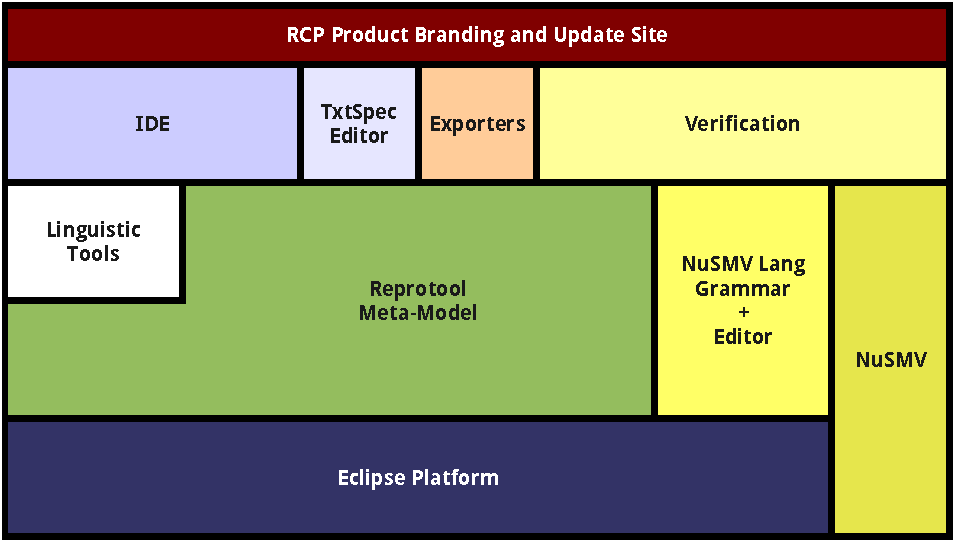
\includegraphics[width=\textwidth]{images/ArchitectureOverview}
  \caption{Reprotool Architecture Overview}
  \label{fig:ArchitectureOverview}
\end{figure}



\subsection{Product Branding}
%TODO: this section is a stub
Everything about branding a standalone RCP application.
\begin{verbatim}
org.eclipselabs.reprotool.branding
org.eclipselabs.reprotool.product
org.eclipselabs.reprotool.target
\end{verbatim}



\subsection{Update Site}
%TODO: this section is a stub
Everything about creating an update site using features.
\begin{verbatim}
org.eclipselabs.reprotool.features.common
org.eclipselabs.reprotool.features.exporters
org.eclipselabs.reprotool.features.ide
org.eclipselabs.reprotool.features.nlp
org.eclipselabs.reprotool.features.verification
\end{verbatim}
